\documentclass[11pt]{article}
\usepackage[english]{babel}
\usepackage[utf8x]{inputenc}
\usepackage{amsmath}
\usepackage{graphicx}
\usepackage[colorinlistoftodos]{todonotes}
\usepackage{enumitem}
\usepackage{listings}
\usepackage{filecontents}
\usepackage{verbatim}
\usepackage{eurosym}
\usepackage[export]{adjustbox}
\usepackage[hidelinks]{hyperref}

\begin{document}

\begin{titlepage}

\newcommand{\HRule}{\rule{\linewidth}{0.5mm}} % Defines a new command for the horizontal lines, change thickness here

\center % Center everything on the page
 
%----------------------------------------------------------------------------------------
%	HEADING SECTIONS
%----------------------------------------------------------------------------------------

\textsc{\LARGE Concordia University}\\[1.5cm] % Name of your university/college
\textsc{\Large COMP 5531 Files and Databases}\\[0.5cm] % Major heading such as course name
%\textsc{\large Assignment 1}\\[0.5cm] % Minor heading such as course title

%----------------------------------------------------------------------------------------
%	TITLE SECTION
%----------------------------------------------------------------------------------------

\HRule \\[0.4cm]
{ \huge \bfseries Main Project Report \\ Web Career Portal Database}\\[0.4cm] % Title of your document
\HRule \\[1.5cm]
 
%----------------------------------------------------------------------------------------
%	AUTHOR SECTION
%----------------------------------------------------------------------------------------

\begin{minipage}{0.4\textwidth}
\begin{flushleft} \large
\emph{Team ID:} \\ cxc55311 \\
\end{flushleft}
\end{minipage}
~
\begin{minipage}{0.4\textwidth}
\begin{flushright} \large
\emph{Team Members:} \\
Md Tanveer Alamgir \\ ID: 40014877\\
Craig Boucher \\ ID: 21295721 \\
Osman Momoh \\ ID: 26220150\\
Fan Zou \\ ID: 40118112\\

\end{flushright}
\end{minipage}\\[2cm]

%\emph{GitHub:} \\ \url{https://github.com/OM234/COMP-5531-Main-Project} \\

% If you don't want a supervisor, uncomment the two lines below and remove the section above
%\Large \emph{Author:}\\
%John \textsc{Smith}\\[3cm] % Your name

%----------------------------------------------------------------------------------------
%	DATE SECTION
%----------------------------------------------------------------------------------------

%{\large \today}\\[2cm] % Date, change the \today to a set date if you want to be precise

%----------------------------------------------------------------------------------------
%	LOGO SECTION
%----------------------------------------------------------------------------------------


\includegraphics[width=50px, keepaspectratio]{Briefcase.png}\\[1cm] % Include a logo
 
%----------------------------------------------------------------------------------------

\vfill % Fill the rest of the page with whitespace

\end{titlepage}

\tableofcontents

\newpage

\section{Introduction}

This project consists of two main components. The design of the database and the website that is used as a tool to implement the database and showcase various features. The database design consisted of creating an entity relation diagram to abstract the database to the core components necessary. This diagram was then used to project the relations that will be required and their associated attributes. From this schema, the functional dependencies were determined and rigorous normalization was performed to ensure the relations were all in at least third normal form. \par
The website, known as the web portal, has a front end to display the user interface and a back-end which connects the functionality between the MySQL database and the front end components. A model-view-controller architecture pattern is used to organize the code in the various files used to build the web portal. \par
The website itself is a career portal interface. There are three types of accounts that have access to the website. Administrators, who have powers to modify other user accounts. Employers, who can post jobs and offer employment. Lastly, job seekers (also known as applicants), can search for job postings and apply to them. The website also handles payment information and payment processing.

\section{Database Design}

The reasonable assumptions made based on the requirements provided in the project description include the following. There will be a table for employers that will contain attributes like the name of the employer, their account category, contact information, username, and password. A table for job seekers (`ordinary' users) to hold data regarding their contact information, account balance, category type, username, and password. A table restricted to administrator accounts will also be necessary. These assumptions were used as a starting point to craft an entity relationship model.

\subsection{Entity-Relation Diagram}

\subsection{E/R Diagram to Relation Conversions}

\subsection{Functional Dependencies}

\subsubsection{Normalization}

\section{Web Portal Functionalities}
Technical languages used: \\
\textit{Programming languages:} JavaScript, PHP, Python \\
\textit{Markup and Stylesheet Languages:} HTML and CSS \\
\textit{Database Management System:} MySQL

\subsection{Software Design \& Architecture}

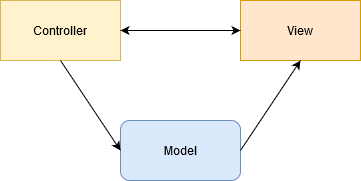
\includegraphics[scale=.7]{MVC.png}

The architectural software design pattern used in the construction of this website is known as Model-View-Controller (MVC). The three interlocking components that perform the core functionality of the website work together to display the interface to the user, gather input from the user, and manage the interaction between the user and the database. The view component displays a graphical interface to the user and receives user input. The controller receives this input and sometimes updates the view directly or manages/manipulates the data requested by the inputs and provides it to the model component. Where the model component, in turn, relays information directly to the view.

\newpage

\subsection{Front-End Development}

Bootstrap, a pivotal framework providing JavaScript and CSS templates was used in the constructions of the front-end. The layout of the website and other visual elements were able to be abstracted away with the Bootstrap framework, making working with the markup and style sheet languages much easier. The functionality for the way users interact with the website were programmed with both JavaScript and PHP.

\subsubsection{Landing Page}

The first page greeting the user is the landing page. Visually, a briefcase image is displayed as a foreground graphic for the website. On the landing page a login request is found. A user can proceed to login, create an account, or request a password if they have forgotten their password. \par
When choosing to create a new account the user will be shown a form to enter various information. All of the fields shown are required. Personal data such as name, email, address, payment information, etc... Will be used to create the new account. If a field is left with an invalid input, the user will be notified to correct any missing information. There are slightly different fields depending on which account type (employer, job seeker) the user chooses to create. \par
The missing password functionality simply sends a password to the email address that is stored on the account. \par
After entering an appropriate username and password the user will be able to login to the website and progress to the dashboard. The dashboard is different for each type of user: job seeker, employer, and administrator (admin).

\subsubsection{Dashboards}

The two main dashboards with most users are the employer and job seeker dashboards. They each provide unique functionalities for the way the user interacts with the website. The third user type, administrators, have unique privilege and access to modify the other user accounts directly. An important feature is that if an account has a negative balance then account becomes frozen and loses access to most features of the website until they provide a payment to obtain a positive balance. \par
The employer dashboard provides the ability to post jobs, update payment information, hire individuals who applied to job postings, delete/deny the applications of job seekers, upgrade the user category (prime, gold), view status of jobs that have been applied to, view posted jobs, update their contact information, and modify payment features. \par 
The job seeker dashboard provides similar features as the employer dashboard such as updating payment information, personal information, and upgrading or downgrading user categories (basic, prime, gold). There is the ability to search for all of the jobs posted in the database. Once a desired job is found, the job seeker user can apply to the job. All of the jobs that have been applied to will be able to be viewed for status updates and whether to accept or reject (withdraw from) job offers. Lastly, the user may delete their account if desired. \par
The last type of account is the administrator. The admins can activate or deactivate any other user (that is not also an admin).  Every job post is also able to be viewed by the admin account.

\subsection{MySQL Database Implementation}

The database management system used is MySQL. A program written in Python was used to generate data to populate the database with. SQL scripts generated by the Python code were then run to create tables and insert the data into the database.

\subsubsection{Generating Data}

A python program was written to generate the data required to fill the database. Everything from phone numbers and email addresses to user names, company names, and credit card numbers were generated using a series of algorithms. Some of the algorithms draw existing data from text files consisting of names, nouns, adjectives, etc... Various forms of primitive data were taken to be used in the algorithms to be combined into data needed to satisfy the attributes belonging to the relations of the database.

\subsubsection{Creating Tables \& Inserting Data}
The files `create\_tables.sql' and `insert\_data.sql' create the database tables and insert the data using SQL queries. The insert data file is generated by the python program. The create table file was written manually based on the database schema provided by the theoretical design work. The primary and foreign keys along with other constraints are clearly implemented in this file.


\subsubsection{SQL Queries}

The file that contains the requested queries is appropriately named `queries.sql'. Some of the queries merely request the manipulation of one record. Such as deleting a user, inserting a user, or posting one job position. All eighteen queries demanded in the main project requirements documented are listed here and labelled with appropriate comments. \par 
The following queries from the requirements document were hand picked to show exactly five tuples, as requested. They were chosen because only these four queries from the document actually demand for a plurality (more than one) tuple. \\
\\
\underline{\textbf{vi.}} Report of posted jobs by an employer during a specific period of time (Job title, date posted, short description, of the job up to 50 characters, number of needed employees to the post, number of applied jobs to the post, number of accepted offers). \\

\begin{verbatim}
SELECT SoJobs, DatePosted, description, EmpNeeded, EmployerName, NumberHired, 
COUNT(SoJobs) as NumberOfApplicants
FROM (SELECT Title as SoJobs, DatePosted, description, EmpNeeded, EmployerName
    FROM employer e join job j on e.UserName = j.EmployerUserName join application
    WHERE EmployerName = 'Ultimate Software' AND (DatePosted BETWEEN '2020-01-26' 
    AND '2020-11-08') and
          application.JobID = j.JobID) as
UltimateSoftwareJobs
join (SELECT a.Title as HireTitle, COUNT(ApplicationStatus) AS NumberHired
FROM (SELECT Title FROM
    employer e join job j on e.UserName = j.EmployerUserName join application
    WHERE EmployerName = 'Ultimate Software' AND (DatePosted BETWEEN '2020-01-26' 
    AND '2020-11-08') and
          application.JobID = j.JobID GROUP BY Title) as a
LEFT JOIN (SELECT Title, ApplicationStatus FROM employer e join job j on 
e.UserName = j.EmployerUserName join application
    WHERE EmployerName = 'Ultimate Software' AND (DatePosted BETWEEN '2020-01-26'
    AND '2020-11-08') and
          application.JobID = j.JobID) as b on a.Title = b.Title and 
          b.ApplicationStatus = 'hired' GROUP BY
          a.Title) as
numberOfHires where UltimateSoftwareJobs.SoJobs = numberOfHires.HireTitle
GROUP BY SoJobs;
\end{verbatim}

\begin{table}[!htbp]
\begin{tabular}{lllllll}
\textbf{Job\_Title}  & \textbf{DatePosted}  & \textbf{EmpNeeded} & \textbf{EmployerName} &  & \\
Electronic Wirer              & 2020-03-27 & 2 & Ultimate Software & 0 & 4 \\
Political Research Scientist  & 2020-08-13 & 4 & Ultimate Software & 0 & 2 \\
Tile-Molder, Hand             & 2020-08-08 & 3 & Ultimate Software & 3 & 7 \\
Jet-Piercer Operator          & 2020-07-13 & 5 & Ultimate Software & 2 & 4 \\
Head of Data                  & 2020-06-17 & 5 & Ultimate Software & 1 & 6 \\
\end{tabular}
\end{table}

$^{*}$\textit{Note}: The job description column is missing from the above table due to not being able to fit on the page. The last two columns are named `NumberHired' and `NumberOfApplicants'.\\

\underline{\textbf{xiii.}} Report of applied jobs by an employee during a specific period of time
(Job title, date applied, short description of the job up to 50 characters,
status of the application).

\begin{verbatim}
SELECT job.Title, application.ApplicationDate, job.description, 
application.ApplicationStatus
FROM application, job
WHERE (ApplicationDate BETWEEN '2020-01-20' AND '2020-10-15') AND 
job.JobID = application.JobID AND
      applicantUserName = 'Bethany_Delena72';
\end{verbatim}

\begin{table}[!htbp]
\begin{tabular}{llll}
\textbf{Job\_Title}                 & \textbf{DateApplied} & \textbf{ApplicationStatus} \\
Machine Joint Cutter                  & 2020-06-20 & denied \\
Green-Chain Offbearer                 & 2020-08-25 & review \\
Womens Health Care Nurse Practitioner & 2020-05-18 & sent   \\
Plan Manager                          & 2020-06-19 & hired  \\
Fish Skinning Machine Feeder          & 2020-06-03 & review \\
\end{tabular}
\end{table}

$^{*}$\textit{Note}: The job description column is missing from the above table due to not being able to fit on the page. 

\newpage

\underline{\textbf{xvii.}} Report of all users by the administrator for employers or employees
(Name, email, category, status, balance).

\begin{verbatim}
SELECT FirstName, LastName, Email, Category, Balance
FROM user natural join applicant
UNION
SELECT FirstName, LastName, Email, Category, Balance
FROM user natural join employer;
\end{verbatim}

\begin{table}[!htbp]
\begin{tabular}{lllll}
\textbf{FirstName}        & \textbf{LastName}          & \textbf{Email} & \textbf{Category}  & \textbf{Balance} \\
Abu          & Llewellyn      & AbuLlewellyn26@coldmail.com          & prime & 264.33 \\
Adolfo       & Shamus         & AdolfoShamus91@hmail.ca              & gold  & 148.68 \\
Aften        & Emmaline       & AftenEmmaline62@hmail.ca             & prime & -55.40 \\
Agatha       & Perfecto       & AgathaPerfecto64@coldmail.com        & prime & 189.96 \\
Ajeenah      & Niclole        & AjeenahNiclole39@coldmail.com        & prime & 47.13  \\
\end{tabular}
\end{table}

\underline{\textbf{xviii.}} Report of all outstanding balance accounts (User name, email, balance,
since when the account is suffering).

\begin{verbatim}
SELECT UserName, email, balance
FROM user
natural join applicant
WHERE balance < 0
UNION
SELECT UserName, email, Balance
from user
natural join employer
WHERE Balance < 0;
\end{verbatim}

\begin{table}[!htbp]
\begin{tabular}{lll}
\textbf{UserName}    & \textbf{Email}        & \textbf{Balance} \\
Daymond\_Zola41     & DaymondZola13@hmail.ca         & -60.39 \\
Jolena\_Collins97   & JolenaCollins79@coldmail.com   & -82.09 \\
Lysander\_Rasean38  & LysanderRasean18@coldmail.com  & -65.59 \\
Naquan\_Madeleine55 & NaquanMadeleine43@coldmail.com & -90.71 \\
Catherina\_Darrol69 & CatherinaDarrol66@hmail.ca     & -62.16
\end{tabular}
\end{table}

\subsection{Back-End Development}

The back back-end provides the interlocking mechanism to link the user interface portion of the web portal with the database. The input provided by the users of the website is acquired and used by the functional capabilities of the back end software to issue queries that retrieve, modify, or insert data into the database. The back-end portion of the website is coded in PHP.

\subsubsection{Sign Up \& Login}

The sign up allows someone to create an employer or job seeker type account. Every field needs to be entered. No empty or inappropriately entered fields will be allowed. Invalid data will not be processed and entered into the database when creating a new account. \par
The login process retrieves the user input from the login fields and verifies the user name and password combination exists in the database. Based on the three different accounts (employer, job seeker, administrator), the appropriate tables are looked at and verified to log into the correct dashboard interface.

\subsubsection{Employer Dashboard}

This dashboard provides features for an employer type account. Jobs that have been posted may be viewed. The employer may also post new jobs for positions they are seeking to fill. The database is asked to retrieve the list of jobs the employer has posted by associating each job with an employer user name (which is a unique identifier for employers). The employer can post many jobs. Therefore, a job identification number and user name combination may be used to retrieve the appropriate list of jobs for each employer user. The employer may also update payment information and the necessary tables are updated in the database when the employer makes this request. \par 
	An employer that is marked as a `prime' category may post up to five jobs. A `gold' category has no limit on the amount of jobs they may post. The database keeps track of these values for each account and updates are made accordingly when an employer type account changes their category. When an employer makes a payment the appropriate amount is deducted from their overall balance, which is also kept track of in the database. \par
	If the balance of an account becomes negative than the account is frozen. The database keeps track of every dollar amount in each account and automatically limits the website functionality for negative balance accounts. These frozen accounts will not have access to any features of the website until enough payments are made to achieve a positive balance.	
	
\subsubsection{Job Seeker Dashboard}

After verifying the login credentials for a job seeker type account based on the user input the user is greeted with the job seeker dashboard. The main features of this dashboard include a searchable database of all jobs that have been posted and the ability to send an application to these jobs. The user can search by job title and job category. The connection with the database allows the appropriate tables to be retrieved based on similarities with the search terms and what is inside the job table attributes. \par 
The job seeker user may also see a list of jobs they have applied for as when they apply for a job a new job an `application' is created and inserted into a table containing all jobs that have been applied to. If the user decides to withdraw their application, a deletion query is sent to the database system to remove the application from the table. When a job application is accepted then the user is hired and the application is marked as `hired' in the database. \par 
There is an option to upgrade a job seeker account category (basic, gold, or prime). The record associated with the user in question is updated as needed. A basic is free account and may view jobs but not send an application. The prime account may send up to five job applications with a ten dollar monthly charge. The gold account has no limit to the amount of jobs they may send applications to and costs twenty dollars a month. When a payment is processed a query is sent to update the database with a deduction in the account balance.

\subsubsection{Administrator Dashboard}

The administrator type account has access to a unique dashboard that has the ability to effect other user type accounts. The administrator can also see every job, employer, and job seeker related data available in the database. The administrator can directly deactivate or activate user accounts and retrieve the data associated with accounts. User accounts may also be deleted by the administrator. \par
	When an account is deactivated it can no longer login to the web portal and a warning message will be displayed to the user.

\newpage 

\section{CONTRIBUTIONS}

The entire project was a group collaboration. Weekly group meetings were held with every group member in attendance. We presented and discussed our work to the group and everyone provided feedback, suggestions, and ideas to implement. The entire main project underwent constant incremental improvement with effort provided from all members. \\
\\
\textbf{Database Design} \\
\textit{Entity-Relation Diagram}: Md Tanveer Alamgir \\
\textit{ER Diagram to Schema Conversion}: Md Tanveer Alamgir \\
\textit{Normalization of the Schema}: Md Tanveer Alamgir \\
\\
\textbf{Front-End Web Portal} \\
\textit{Land Page Design \& Interaction}: Osman Momoh \\
\textit{Dashboard Designs \& Interaction}: Osman Momoh \\
\\
\textbf{MySQL Database Implementation}\\
\textbf{\textit{Data Generation Script}}: \par
Design and Construction of Algorithms: Craig Boucher \par
Code Organization with Object-Oriented Design: Osman Momoh \\
\textit{Table Creation, Data Insertion, and Queries}: Craig Boucher \\
\\
\textbf{Back-End Web Portal} \\
\textit{Sign Up \& Login Functionality}: Fan Zou \\
\textit{Employer \& Job Seeker Dashboard Functionality}: Fan Zou \\
\textit{Administrator Dashboard Functionality}: Fan Zou \\
\\
\textbf{Project Report} \\
\textit{Writing, Editing, and Organizing the Report}: Craig Boucher

\end{document}